% mainfile: ../ltexpprt.tex
%In \cite{ref4}
%different types of analysis are used including spatial, temporal, and
%textual analysis. The purpose of spatial analysis is to determine the
%distribution of disease in US while temporal analysis is used for
%tracking the changes in number of tweets with specific keywords.
%Furthermore, text mining is used for tracking the popularity of disease
%types, symptoms, and treatments. Results of these analyses are
%visualized separately and can be used by healthcare officials. An almost
%similar approach was reported in \cite{ref7} that uses spatio-temporal
%analysis of Twitter data to monitor West Nile Virus. 

\begin{figure}[t] \centering
    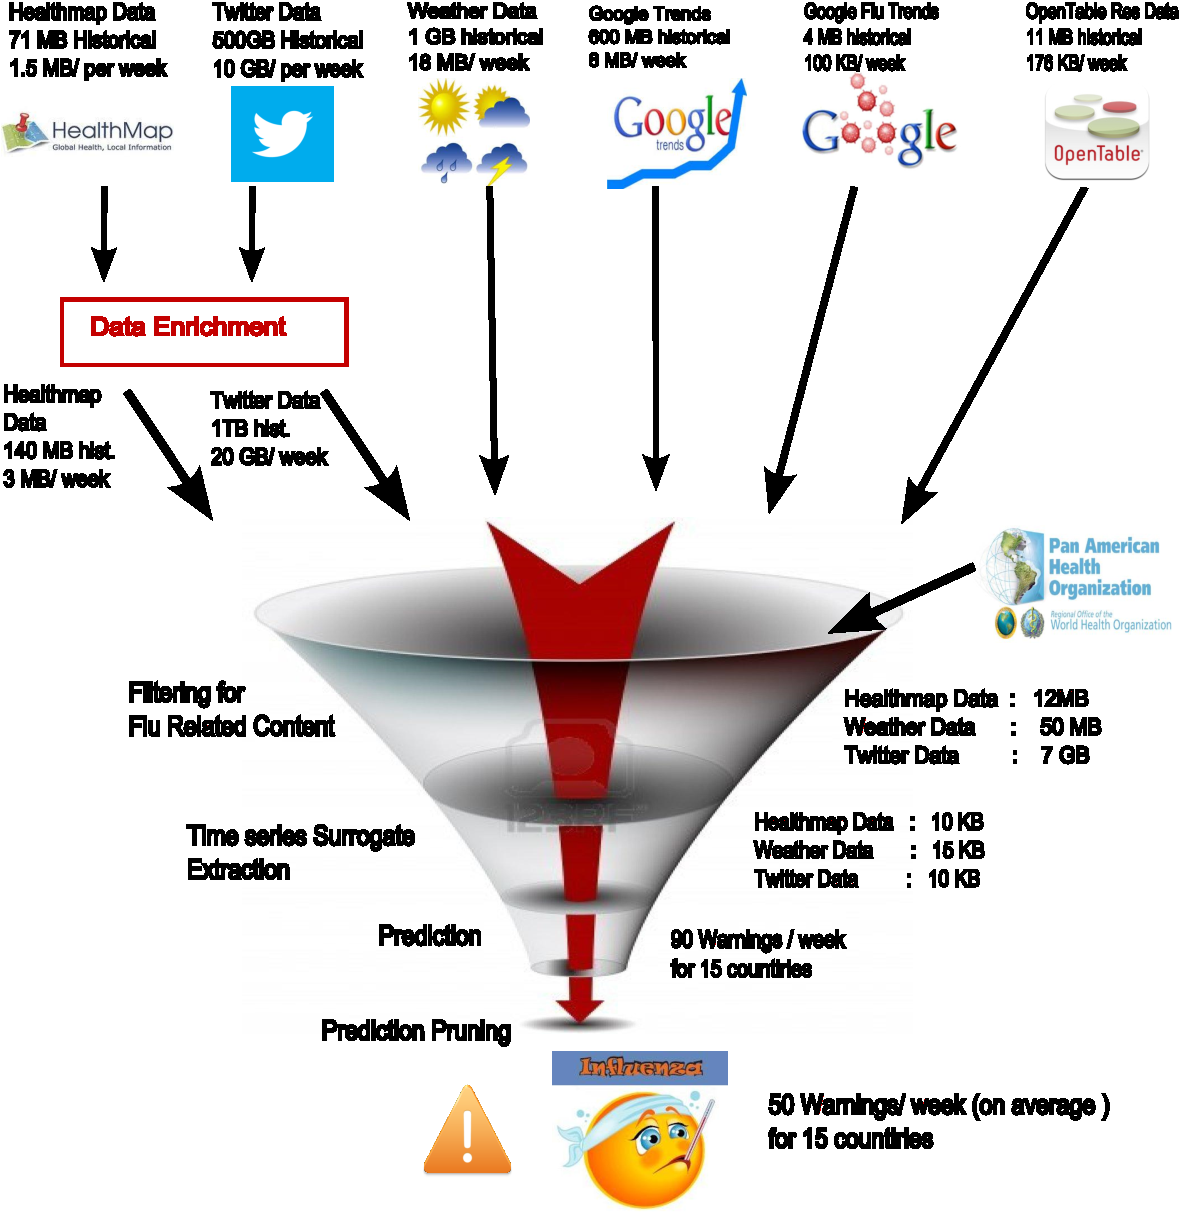
\includegraphics[width=0.95\columnwidth]{fig/ili_data_pipeline.pdf}
    \caption{\label{fig:ili_data_pipeline} Our ILI data pipeline, depicting 
six different data sources used in this paper to forecast ILI case counts.}
 \end{figure}

Related work naturally falls into the categories of social media
analytics, physical indicators, and event dynamics modeling. 
 
\textbf{Social media analytics:}
Most work in social media analytics focuses on Twitter, specifically tracking
a dictionary of ILI-related keywords in the data stream.
Some investigations have focused on the importance of diversity in keyword 
lists, e.g.,~\cite{ref5, ref6}. In~\cite{ref5}, 
Kanhabua and Nejdl used clustering methods to determine
important topics in Twitter data, construct time series for matched keywords,
and used Jaccards coefficient to characterize the temporal
diversity of tweets. They note that such temporal diversity may be
correlated with real-world ILI outbreaks. In~\cite{ref6}
the authors study the dynamics of changes in tweets related to the H1N1 virus. We 
present our approach towards creating the keyword dictionary in Section~\ref{sec:keyword}.

\textbf{Physical indicators for detecting ILI incidence levels:} 
%One of the key indicators of ILI levels in a country is the prevalent 
%climactic patterns and the deviation from ``normal'' levels of these 
%indicators. For example 
Tamerius et al.~\cite{ref9} investigated the existence of seasonal 
cycles of influenza epidemics in different climate regions
by considering climatic information from 78 globally distributed sites. Through 
logistic regression they found that, in cold-dry and humid-rainy
environments, strong correlation exists between influenza epidemics and
weather conditions. Similary exciting results were found 
by Shaman et. al.~\cite{Shaman_orig_humidity_link, Shaman_humidity_USA}
where they discovered absolute humidity to be a key indicator of flu. To uncover 
these relationships they used non-linear regressors such as Kalman filters,
and this was a key inspiration to us to find a uniform model for the
vaired data sources as explained in Section~\ref{sec:methods}.

%\textbf{Non-linear regression methods:}
%There has been significant research in recommender systems to predict unknown user 
%ratings by combining techniques such as
%matrix factorization and nearest neighbor modeling. Although
%working essentially on categorical data, these methods are fine examples of non-linear
%regression methods which have been found to be robust as well as scalable (see~\cite{koren2008factor}).
%While matrix factorization have been long used (see ~\cite{canny2002factor}) to 
%connect the independent and dependent variables through latent factors, 
%recently Koren et al.~\cite{koren2008factor} presented detailed comparisons
%of nearest neighbors with matrix factorization methods and provided frameworks to 
%integrate the two approaches towards a unified non-linear predictor.
%
\textbf{Event dynamics modeling:}
Denecke et al.~\cite{ref3}
have proposed an event-based approach for early prediction
of ILI threats \cite{ref3}. In their method (M-Eco) they consider
multiple resources such as Twitter, TV reports, online news articles,
and blogs. M-Eco is a bi-lingual system that works with information in
English and German and uses clustering to identify signals for event detection.
%Also, there exists related research in modeling the progression of influenza epidemics using
%dynamical systems. 
Network dynamic solutions are used in~\cite{ref11} 
to study the behavior of an epidemic in a society. Spread of an infection through a network 
has been also studied as a general problem in graph mining, e.g., see~\cite{ref14}.
 
